\begin{center}
    \begin{figure}[H]
        \centering

        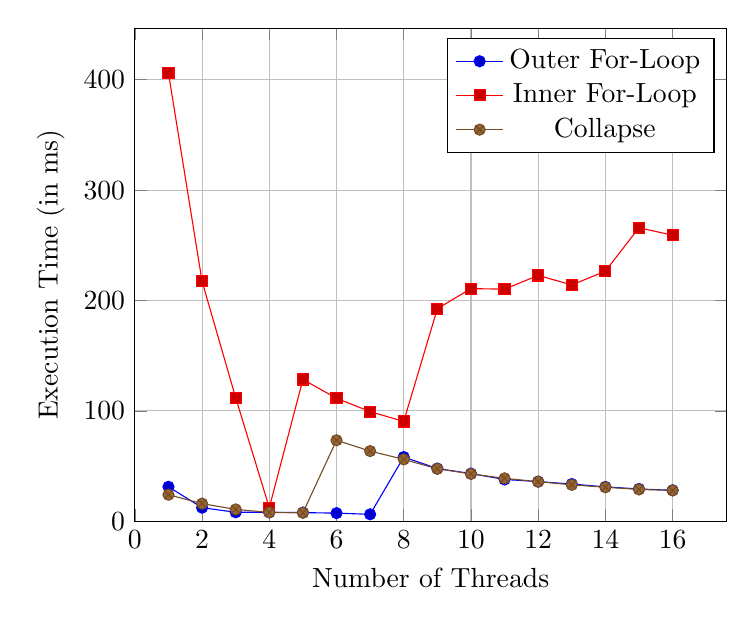
\begin{tikzpicture}
            \begin{axis}[
                title={},
                width=0.75\textwidth,
                xlabel={Number of Threads},
                ylabel={Execution Time (in ms)},
                xmin=0,
                ymin=0,
                grid=major
            ]
                \addplot coordinates {
                    (1,31.2605)(2,12.3476)(3,8.17925)(4,8.15845)(5,7.901)(6,7.3853)(7,6.33095)(8,58.2227)(9,47.7963)(10,43.2362)(11,37.9023)(12,35.9582)(13,33.7485)(14,31.185)(15,29.2952)(16,28.0915)
                };
                \addlegendentry{Outer For-Loop}

                \addplot coordinates {
                    (1,406.043)(2,217.313)(3,111.939)(4,12.3023)(5,128.511)(6,111.441)(7,99.3506)(8,90.4608)(9,192.601)(10,210.794)(11,210.268)(12,222.735)(13,214.113)(14,226.578)(15,265.97)(16,259.109)
                };
                \addlegendentry{Inner For-Loop}       

                \addplot coordinates {
                    (1,24.0952)(2,16.0462)(3,10.7771)(4,8.0282)(5,7.75735)(6,73.4093)(7,63.6226)(8,56.107)(9,47.5841)(10,42.9433)(11,38.9119)(12,35.9038)(13,33.0421)(14,30.8513)(15,28.8692)(16,27.9851)
                };
                \addlegendentry{Collapse}
            \end{axis}
        \end{tikzpicture}
        \caption{Grayscale Performance Tests pnglogo-blk.png}
    \end{figure}
\end{center}